\chapter{TEST APPENDICES}

Node.js is an open source and cross platform JavaScript runtime environment [5]. Node.js allows developers to use JavaScript to write the command line tools and for server-side scripting to produce dynamic web page content before the page publishes to the users’ web browser.

\section{Figure}
Node.js is an asynchronous event-driven JavaScript runtime which is designed to build scalable network applications. It runs with the V8 JavaScript engine outside of the browser. Therefore, Node.js becomes very performant.

\begin{figure}[htbp]
    \centering
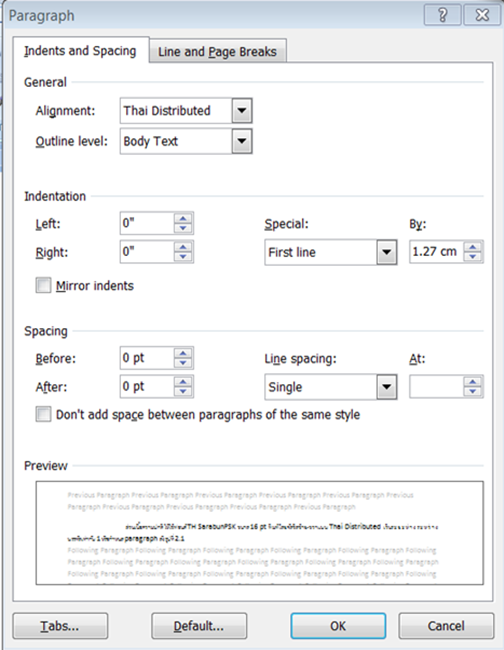
\includegraphics[width = 0.5\textwidth]{paragraph.png}
    \caption{Paragraph arrangement}
    \label{fig:paragraph}
\end{figure}

\subsection{Equation}
Node.js is an asynchronous event-driven JavaScript runtime which is designed to build scalable network applications. It runs with the V8 JavaScript
\begin{equation}
E=mc^{2}
\end{equation}
นิยมวางสมการไว้กึ่งกลางหน้ากระดาษ และหมายเลขสมการพิมพ์ชิดขวา

\subsubsection{Coding}
Node.js is an asynchronous event-driven JavaScript runtime which is designed to build scalable network applications. It runs with the V8 JavaScript 

\begin{lstlisting}[language=C]
public static void main(String[] args)
{
	System.out.println(“Hello World”);
}
\end{lstlisting}
\section{Table}
GraphQL is both an API query language and a runtime for executing those queries using your current data. GraphQL allows clients the power to ask for exactly what they need and nothing more, makes it easier to evolve APIs over time, and enables powerful developer tools by providing a clear and intelligible description of the data in your API
\begin{table}[hbt!]
    \caption{ตารางข้อมูลตัวอย่าง}
    \centering
    \begin{tabularx}{\textwidth}{|Y|Y|Y|Y|}
    \hline
       ลำดับที่ & ตัวแปร & ค่าของตัวแปร & ตัวอย่าง  \\
    \hline
        1 & $x$ & 15 & $x=15$\\
    \hline
        2 & $y$ & 30 & $y=30$\\
    \hline
    \end{tabularx}
    \label{tab:my_label}
\end{table}

\subsection{Equation}
Node.js is an asynchronous event-driven JavaScript runtime which is designed to build scalable network applications. It runs with the V8 JavaScript
\begin{equation}
E=mc^{2}
\end{equation}
นิยมวางสมการไว้กึ่งกลางหน้ากระดาษ และหมายเลขสมการพิมพ์ชิดขวา

\subsubsection{Coding}
Node.js is an asynchronous event-driven JavaScript runtime which is designed to build scalable network applications. It runs with the V8 JavaScript 

\begin{lstlisting}[language=C]
public static void main(String[] args)
{
	System.out.println(“Hello World”);
}
\end{lstlisting}
\section{Table}
GraphQL is both an API query language and a runtime for executing those queries using your current data. GraphQL allows clients the power to ask for exactly what they need and nothing more, makes it easier to evolve APIs over time, and enables powerful developer tools by providing a clear and intelligible description of the data in your API
\begin{table}[hbt!]
    \caption{ตารางข้อมูลตัวอย่าง}
    \centering
    \begin{tabularx}{\textwidth}{|Y|Y|Y|Y|}
    \hline
       ลำดับที่ & ตัวแปร & ค่าของตัวแปร & ตัวอย่าง  \\
    \hline
        1 & $x$ & 15 & $x=15$\\
    \hline
        2 & $y$ & 30 & $y=30$\\
    \hline
    \end{tabularx}
    \label{tab:my_label}
\end{table}